\documentclass[12pt]{article}
\usepackage[utf8]{inputenc}
\usepackage{float}
\usepackage{amsmath}
\usepackage{tikz}

\usepackage[hmargin=3cm,vmargin=6.0cm]{geometry}
%\topmargin=0cm
\topmargin=-2cm
\addtolength{\textheight}{6.5cm}
\addtolength{\textwidth}{2.0cm}
%\setlength{\leftmargin}{-5cm}
\setlength{\oddsidemargin}{0.0cm}
\setlength{\evensidemargin}{0.0cm}

%misc libraries goes here



\begin{document}

\section*{Student Information } 
%Write your full name and id number between the colon and newline
%Put one empty space character after colon and before newline
Full Name : Ersel Hengirmen \\
Id Number : 2468015 \\

% Write your answers below the section tags
\section*{Answer 1}
a) Hasse below:\\
\begin{figure}[H]
	\centering
	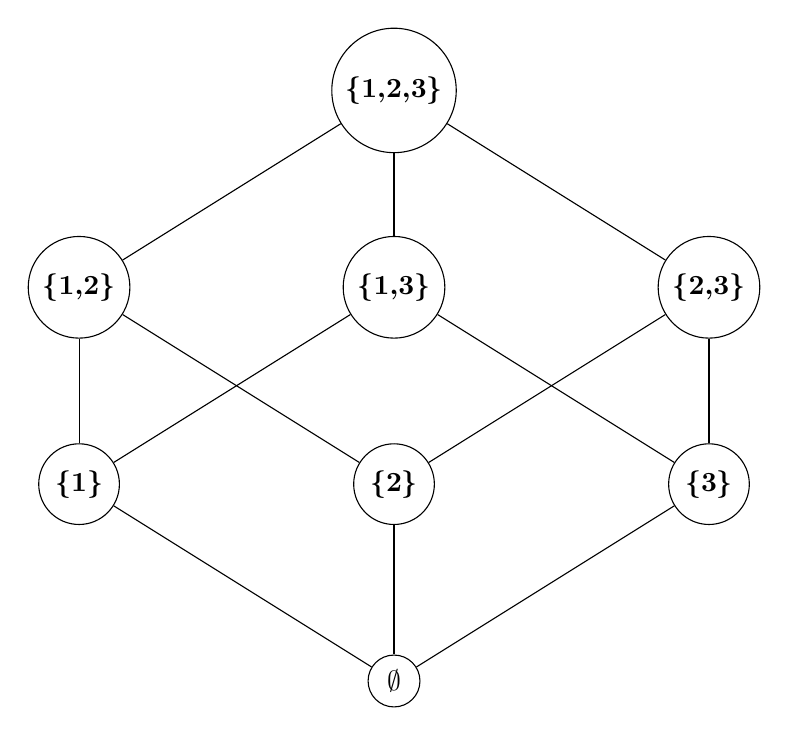
\begin{tikzpicture}
	
	\node[shape=circle,draw=black] (a) at (7, 7.5)     {\textbf{\{1,2,3\}}};
	\node[shape=circle,draw=black] (b) at (3, 5)     {\textbf{\{1,2\}}};
	\node[shape=circle,draw=black] (c) at (7, 5)     {\textbf{\{1,3\}}};
	\node[shape=circle,draw=black] (d) at (11, 5)     {\textbf{\{2,3\}}};
	\node[shape=circle,draw=black] (e) at (3, 2.5)     {\textbf{\{1\}}};
	\node[shape=circle,draw=black] (f) at (7, 2.5)     {\textbf{\{2\}}};
	\node[shape=circle,draw=black] (g) at (11, 2.5)     {\textbf{\{3\}}};
	\node[shape=circle,draw=black] (h) at (7, 0)     {\textbf{$\emptyset$}};
	
	\path[-] (a) edge (b);
	\path[-] (a) edge (c);
	\path[-] (a) edge (d);
	\path[-] (b) edge (e);
	\path[-] (b) edge (f);
	\path[-] (c) edge (e);
	\path[-] (c) edge (g);
	\path[-] (d) edge (f);
	\path[-] (d) edge (g);
	\path[-] (e) edge (h);
	\path[-] (f) edge (h);
	\path[-] (g) edge (h);
	
	\end{tikzpicture} 
	\label{fig:t6}
\end{figure}
b) It is a lattice. Because every 2 elements has LUB and GLB\\
\\
c)It has only 1 maximal element which is \{1,2,3\}\\
\\
d)It has only 1 minimal element which is $\emptyset$ \\
\\
e)Yes there is a greatest element and it is \{1,2,3\} \\
\\
f)Yes there is a least element and it is $\emptyset$\\
\\
g) LUB of \{1\} and \{3\} is \{1,3\}\\

\section*{Answer 2}
a)There are 7 edges each edge will increase the degree of its vertexes by 1 which means sum of all degrees is 7*2=14\\
\\
b)Number of non-zero entries in the adjacency matrix representation of G can be easily found once again by:\\
$2*edge\_count=2*7=14$\\
This is so since every connection will be represented by 1 edge on the graph and every edge will represent 2 points(unless there is a self edge).\\
\\
c)Incidince matrix will set first and second vertexes of an edge as 1. For every other vertex 0. And it will be done for every edge. That means once again we will have 2*7=14 non-zero entries\\
d)Yes it does nultiple in fact. Lets show only one of them:\\
\begin{figure}[H]
	\centering
	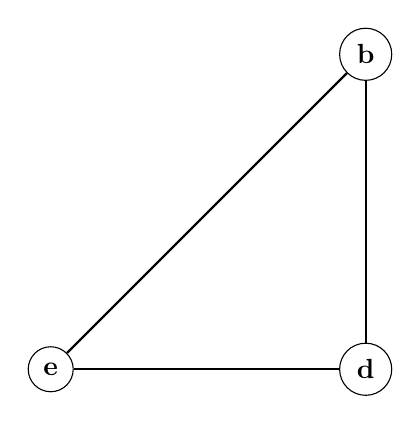
\begin{tikzpicture}
	
	\node[shape=circle,draw=black] (b) at (4, 4)     {\textbf{b}};
	\node[shape=circle,draw=black] (d) at (4, 0)     {\textbf{d}};
	\node[shape=circle,draw=black] (e) at (0, 0)     {\textbf{e}};
	
	\path[-, thick] (b) edge (e);
	\path[-, thick] (b) edge (d);
	\path[-, thick] (d) edge (e);
	
	\end{tikzpicture} 
	\label{fig:g2}
\end{figure}
e)It is not a bipartite graph because its chromatic number is not 2 but 3. Since its chromatic number is 3 if we tried to put its vertexes in 2 parts at least one of the vertexes would be connected to 1 vertex from both parts. Because of that it cant be a bipartate graph\\
By the way if there is at least one simple circuit with odd number of nodes in your graph then that graph's chromatic number will be at least 3 and because of that it wont be able to be a bipartite graph.\\
The bipartate subgraph is below:\\
\begin{figure}[H]
	\centering
	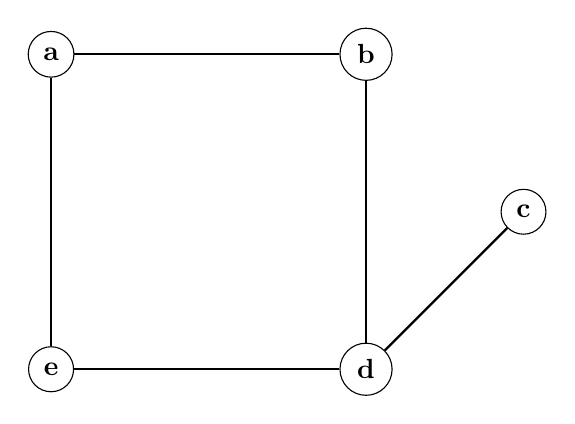
\begin{tikzpicture}
	
	\node[shape=circle,draw=black] (a) at (0, 4)     {\textbf{a}};
	\node[shape=circle,draw=black] (b) at (4, 4)     {\textbf{b}};
	\node[shape=circle,draw=black] (c) at (6, 2)     {\textbf{c}};
	\node[shape=circle,draw=black] (d) at (4, 0)     {\textbf{d}};
	\node[shape=circle,draw=black] (e) at (0, 0)     {\textbf{e}};
	
	\path[-, thick] (a) edge (b);
	\path[-, thick] (a) edge (e);
	\path[-, thick] (b) edge (d);
	\path[-, thick] (d) edge (c);
	\path[-, thick] (d) edge (e);
	
	\end{tikzpicture} 
	\label{fig:g2}
\end{figure}
f) It has 2 situations:\\
1-either edge(v1,v2) will be from v1 to v2\\
2-or v2 to v1\\
\\
that means we will have $2^7=128$ different directed graphs that have G as their underlying undirected graph\\
\\
g)length of the simple longest path can be at most 4 since we have 5 vertexes. This is because we can go to a vertex at most once. And simple longest path actually is 4\\
a,b,c,d,e is one of the longest simple paths.\\
\\
h)It is 1 since everything is connected so we can reach every vertex from every other vertex.\\
\\
i)There isn't an euler circuit since not every one of the vertexes have even degrees. vertexes d and e has 3 edges.\\
\\
j)There is an euler path since a total of 2 vertexes has odd degrees(path will start and end in them) and others have even. The eular path is:\\ e,a,b,c,d,e,b,d\\
\\
k)Yes it has a Hamilton circuit, a,b,c,d,e,a\\
\\
l)Yes it has a Hamilton path, a,b,c,d,e\\

\section*{Answer 3}	
They are isomorphic since we can connect them like:\\
a$\rightarrow$a’\\
c$\rightarrow$e’\\
\\
b$\rightarrow$c’\\
d$\rightarrow$g’\\
\\
e$\rightarrow$b’\\
f$\rightarrow$h’\\
\\
g$\rightarrow$d’\\
h$\rightarrow$f’\\
\\
And we can connect them like that because:\\
1-For a$\rightarrow$a’:\\
a is connected to\\
b,d,e,f\\
and their corresponding points on H are:\\
c’,g’,b’,h’ in this order which are all connected to a’\\
\\
2-For c$\rightarrow$e’\\
c is connected to\\
b,d,g,h\\
and their corresponding points on H are:\\
c’,g’,d’,f’ in this order which are all connected to e’\\
\\
3-For b$\rightarrow$c’\\
b is connected to\\
a,c,e,g\\
and their corresponding points on H are:\\
a’,e’,b’,d’ in this order which are all connected to c’\\
\\
4-For d$\rightarrow$g’\\
d is connected to\\
a,c,f,h\\
and their corresponding points on H are:\\
a’,e’,h’,f’ in this order which are all connected to g’\\
\\
5-For e$\rightarrow$b’\\
e is connected to\\
a,b,f,h\\
and their corresponding points on H are:\\
a’,c’,h’,f’ in this order which are all connected to b’\\
\\
6-For f$\rightarrow$h’\\
f is connected to\\
a,d,e,g\\
and their corresponding points on H are:\\
a’,g’,b’,d’ in this order which are all connected to h’\\
\\
7-For g$\rightarrow$d’\\
g is connected to\\
b,c,f,h\\
and their corresponding points on H are:\\
c’,e’,h’,f’ in this order which are all connected to d’\\
\\
8-For h$\rightarrow$f’\\
h is connected to\\
c,d,e,g\\
and their corresponding points on H are:\\
e’,g’,b’,d’ in this order which are all connected to f’\\
\\
Since above transformation holds they are isomorphic.

\section*{Answer 4}
At first we will denote distance of every vertex from starting vertex(a) as $\infty$ except for our starting vertex(a). We will denote starting vertex's(a) distance to itself as 0 and then at every turn we will choose the vertex that has the lowest distance to starting vertex(a) which hasn't been already chosen. and we will look at its neighbors; if its neighbor's original distance is higher then:\\
(current vertex's distance to vertex a+current vertex's distance to its neighbor)\\
then we will denote that neighbor's distance to our starting vertex(a) as (current vertex's distance to vertex a+current vertex's distance to its neighbor).\\
\\
\textbf{Important Note:} Since chosen nodes are already has the lowest distance(since there are no negative edges and since we are choosing lowest distanced vertex every time) we dont have to compare them anymore. And also we can stop when we choose j since we would have found its lowest distance at that time.\\
\\
Now lets start:\\
\begin{table}[H]
	\centering
	\begin{tabular}{|l| c | c | c | c | c | c | c | c | c | c | c |}
		\hline
		chosen\textbackslash distance& a & b & c & d & e & f & g & h & i & j & k \\ \hline
		NONE & 0 & $\infty$ & $\infty$ & $\infty$ & $\infty$ & $\infty$ & $\infty$ & $\infty$ & $\infty$ & $\infty$ & $\infty$ \\ \hline
		
		 \textbf{a} & \textcolor{red}{\textbf{0}} & 3 & $\infty$ & $\infty$ & 5 & $\infty$ & $\infty$ & 4 & $\infty$ & $\infty$ & $\infty$ \\ \hline
		
		a,\textbf{b} & \textbf{0} & \textcolor{red}{\textbf{3}} & 5 & $\infty$ & 5 & 10 & $\infty$ & 4 & $\infty$ & $\infty$ & $\infty$ \\ \hline
		
		a,b,\textbf{h} & \textbf{0} & \textbf{3} & 5 & $\infty$ & 5 & 9 & $\infty$ & \textcolor{red}{\textbf{4}} & 6 & $\infty$ & $\infty$ \\ \hline
		
		a,b,h,\textbf{c} & \textbf{0} & \textbf{3} & \textcolor{red}{\textbf{5}} & 8 & 5 & 7 & 11 & \textbf{4} & 6 & $\infty$ & $\infty$ \\ \hline
		
		a,b,h,c,\textbf{e} & \textbf{0} & \textbf{3} & \textbf{5} & 8 & \textcolor{red}{\textbf{5}} & 7 & 11 & \textbf{4} & 6 & $\infty$ & $\infty$ \\ \hline
		
		a,b,h,c,e,\textbf{i} & \textbf{0} & \textbf{3} & \textbf{5} & 8 & \textbf{5} & 7 & 11 & \textbf{4} & \textcolor{red}{\textbf{6}} & 12 & $\infty$ \\ \hline
		
		a,b,h,c,e,i,\textbf{f} & \textbf{0} & \textbf{3} & \textbf{5} & 8 & \textbf{5} & \textcolor{red}{\textbf{7}} & 11 & \textbf{4} & \textbf{6} & 10 & $\infty$ \\ \hline
		
		a,b,h,c,e,i,f,\textbf{d} & \textbf{0} & \textbf{3} & \textbf{5} & \textcolor{red}{\textbf{8}} & \textbf{5} & \textbf{7} & 11 & \textbf{4} & \textbf{6} & 10 & 10 \\ \hline
		
		
	\end{tabular}
\end{table}
operations at each step:\\
\\
Step-1:(chosen vertex:a(3 edges))\\
b$\rightarrow$min($\infty$,0+3)=3\\
e$\rightarrow$min($\infty$,0+5)=5\\
h$\rightarrow$min($\infty$,0+4)=4\\
\\
Step-2:(chosen vertex:b(4 edges))\\
a was already chosen\\
c$\rightarrow$min($\infty$,3+2)=5\\
e$\rightarrow$min(5,3+5)=5\\
f$\rightarrow$min($\infty$,3+7)=10\\
\\
Step-3:(chosen vertex:h(4 edges))\\
a was already chosen\\
e$\rightarrow$min(5,4+7)=5\\
f$\rightarrow$min(10,4+5)=9\\
i$\rightarrow$min($\infty$,4+2)=6\\
\\
Step-4:(chosen vertex:c(4 edges) (we could have also chosen e))\\
a was already chosen\\
d$\rightarrow$min($\infty$,5+3)=8\\
f$\rightarrow$min(9,5+2)=7\\
g$\rightarrow$min($\infty$,5+6)=11\\
\\
Step-5:(chosen vertex:e(4 edges))\\
a was already chosen\\
b was already chosen\\
h was already chosen\\
f$\rightarrow$min(7,5+4)=7\\
\\
Step-6:(chosen vertex:i(3 edges))\\
h was already chosen\\
f$\rightarrow$min(7,6+4)=7\\
j$\rightarrow$min($\infty$,6+6)=12\\
\\
Step-7:(chosen vertex:f(7 edges))\\
b was already chosen\\
c was already chosen\\
e was already chosen\\
h was already chosen\\
i was already chosen\\
g$\rightarrow$min(11,7+4)=11\\
j$\rightarrow$min(12,7+3)=10\\
\\
Step-8:(chosen vertex:d(3 edges))\\
c was already chosen\\
g$\rightarrow$min(11,8+7)=11\\
k$\rightarrow$min($\infty$,8+2)=10\\
\\
Step-9 chosen vertex is j so distance to j from a is \textbf{10}\\

\section*{Answer 5}
I have chosen \textbf{Kruskal}.\\
\\
a)\\
1-Edge(a,b)\\
2-Edge(c,e)\\
3-Edge(e,f)\\
we are not gonna choose edge(f,c) since it would create a circuit\\
4-Edge(a,d)\\
5-Edge(b,c)\\
\\
b) one of the possible minimum spanning trees:\\
\begin{figure}[H]
	\centering
	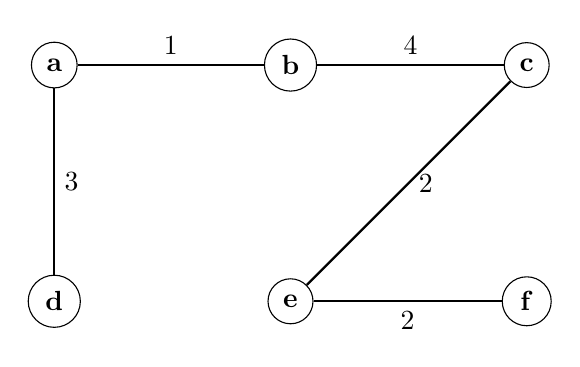
\begin{tikzpicture}
	
	\node[shape=circle,draw=black] (a) at (0, 3)     {\textbf{a}};
	\node[shape=circle,draw=black] (b) at (3, 3)     {\textbf{b}};
	\node[shape=circle,draw=black] (c) at (6, 3)     {\textbf{c}};
	\node[shape=circle,draw=black] (d) at (0, 0)     {\textbf{d}};
	\node[shape=circle,draw=black] (e) at (3, 0)     {\textbf{e}};
	\node[shape=circle,draw=black] (f) at (6, 0)     {\textbf{f}};
	
	\path[-, thick] (a) edge node[above]{1} (b);
	\path[-, thick] (b) edge node[above]{4} (c);
	\path[-, thick] (a) edge node[right]{3} (d);
	\path[-, thick] (c) edge node[right]{2} (e);
	\path[-, thick] (e) edge node[below]{2} (f);
	
	\end{tikzpicture} 
	\label{fig:g5}
\end{figure}
c) It is not because there are 2 more which are:\\
\begin{figure}[H]
	\centering
	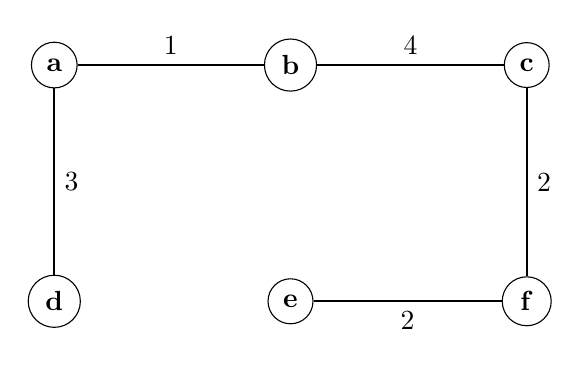
\begin{tikzpicture}
	
	\node[shape=circle,draw=black] (a) at (0, 3)     {\textbf{a}};
	\node[shape=circle,draw=black] (b) at (3, 3)     {\textbf{b}};
	\node[shape=circle,draw=black] (c) at (6, 3)     {\textbf{c}};
	\node[shape=circle,draw=black] (d) at (0, 0)     {\textbf{d}};
	\node[shape=circle,draw=black] (e) at (3, 0)     {\textbf{e}};
	\node[shape=circle,draw=black] (f) at (6, 0)     {\textbf{f}};
	
	\path[-, thick] (a) edge node[above]{1} (b);
	\path[-, thick] (b) edge node[above]{4} (c);
	\path[-, thick] (a) edge node[right]{3} (d);
	\path[-, thick] (c) edge node[right]{2} (f);
	\path[-, thick] (e) edge node[below]{2} (f);
	
	\end{tikzpicture} 
	\label{fig:g5}
\end{figure}

\begin{figure}[H]
	\centering
	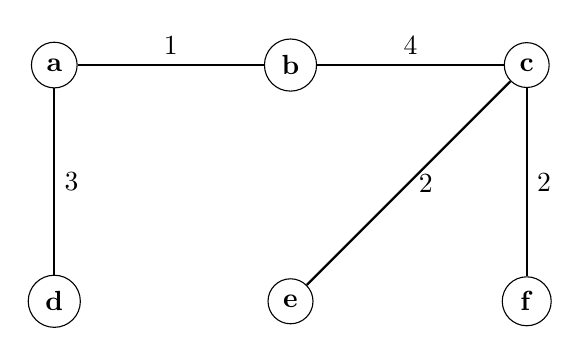
\begin{tikzpicture}
	
	\node[shape=circle,draw=black] (a) at (0, 3)     {\textbf{a}};
	\node[shape=circle,draw=black] (b) at (3, 3)     {\textbf{b}};
	\node[shape=circle,draw=black] (c) at (6, 3)     {\textbf{c}};
	\node[shape=circle,draw=black] (d) at (0, 0)     {\textbf{d}};
	\node[shape=circle,draw=black] (e) at (3, 0)     {\textbf{e}};
	\node[shape=circle,draw=black] (f) at (6, 0)     {\textbf{f}};
	
	\path[-, thick] (a) edge node[above]{1} (b);
	\path[-, thick] (b) edge node[above]{4} (c);
	\path[-, thick] (a) edge node[right]{3} (d);
	\path[-, thick] (c) edge node[right]{2} (e);
	\path[-, thick] (c) edge node[right]{2} (f);
	
	\end{tikzpicture} 
	\label{fig:g5}
\end{figure}
\section*{Answer 6}
a)\\
Number of vertices:13\\
Number of edges:12\\
Height:4\\
\\ 
b)In postorder we use left-right-root for every subtree\\
the order is: w,s,m,t,q,x,n,y,u,z,v,r,p\\
\\
c)In inorder we use left-root-right for every subtree\\
the order is: s,w,q,m,t,p,x,u,n,y,r,v,z\\
\\
d)In preorder we use root-left-right for every subtree\\
the order is: p,q,s,w,t,m,r,u,x,y,n,v,z\\
\\
e) T is not a full binary tree since some of its nodes has exactly one child for example:\\
node s has only right-child w and no left child.\\


\end{document}